\chapter{Project Management}

\section{Project organisation and tools}

\subsection{GitLab}

GitLab is arguably the best tool out there for common DevOps practices. We needed not to expose the original code and the CI. Since CSG offers a protected version of it behind LDAP identification our supervisor and us deemed it suited for our use case. At the start of the group project we started by importing the Voodoo project from our supervisor's private Github and forked the mirror of the Calcite project and imported it in GitLab. We now have 8 projects in GitLab, 5 of which are archived spike projects or different projects that had crossed path with Voodoo (where results of analyses could have been useful).

\paragraph{Version control}
Since we are using Git as our version control, we decided to use \textit{feature branches} - when we are e.g. developing a feature or fixing a certain issue, we create a branch specific to that issue (and not work directly on our main branch). Once our changes are pushed and the CI build is successful (see below), then we can create a merge request into the main branch. These are reviewed by other team members to ensure our code quality, style and correctness is satisfactory, and then merged into main branch.

\paragraph{Continuous Integration}
Once a team member pushes a commit, we automatically build and test the project to ensure quality and keep master branches healthy (see Fig \ref{fig:calcite-pipeline}). Our CI server is an instance of an Apache CloudStack virtual machine provided by the Department of Computing that is protected behind the Imperial firewall and which CPU supports OpenCL. The VM only has Docker installed since we use Docker containers to run the CI. GitLab has a lot of very powerful CI features like caching which we needed to speed up builds and releasing artifacts under a fixed job URL which helped with integration tests. We used the CI as an entry point in the usability objective we had as discussed in more details here.

\begin{figure}[h]
    \centering
    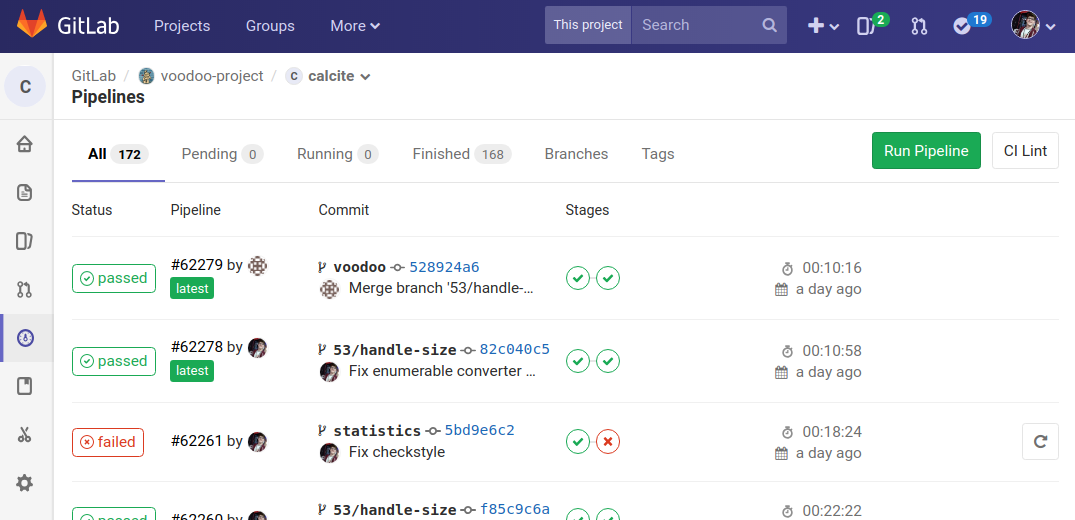
\includegraphics[width=0.98\linewidth, trim={0 0 6cm 7cm}, clip]{project-management/pipeline.png}
    \caption{A list of CI pipelines for the \texttt{calcite} repository}
    \label{fig:calcite-pipeline}
\end{figure}

\paragraph{Issues - Board structure}
GitLab has the most complete issue system, offering so many features to work with merge requests, CI, and also to work on several repositories. It also provides a very functional board system (Figure \ref{fig:gitlab-issues}) that helped to understand at anytime the progress in the checkpoint and to pick up issues that we divided in the following sections:

\begin{itemize}\itemsep0.2em
    \item \textbf{Backlog}: issues with a low level of priority
    \item \textbf{To Do}: issues which need to be completed in this iteration, but not being worked on yet
    \item \textbf{Doing}: issues which some team member(s) are currently working on
    \item \textbf{Closed}: issues which are completed, and the relevant merge requests have been reviewed and merged
\end{itemize}

\begin{figure}[h]
    \centering
    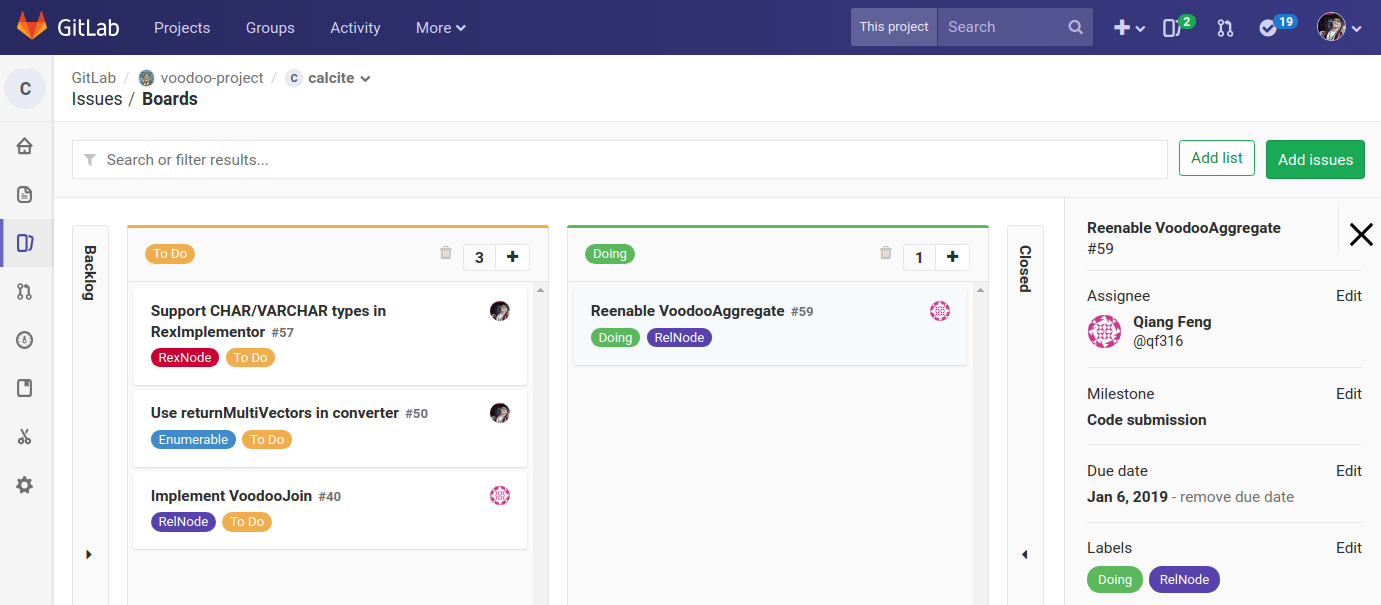
\includegraphics[width=0.98\linewidth, trim={0 0 0 7cm}, clip]{project-management/gitlab-issues.png}
    \caption{Gitlab issues board for our \texttt{calcite} repository}
    \label{fig:gitlab-issues}
\end{figure}

\subsection{Slack}

We decided to use Slack (see Figure \ref{fig:slack}) for online communication since our supervisor was familiar with it.
We kept him updated on the status of the project, and also asked him questions when needed. This turned out to be very useful, especially for the back-end where he could provide details about the existing implementation and explain the Voodoo paper or give us related papers to read.

Slack allows us to have different \emph{channels} so that we can categorise our communications according to which aspect of the project we are discussing. In our case, we have the channels:

\begin{itemize}
    \item \texttt{\#frontend} for communications related to building our Calcite front-end
    \item \texttt{\#codegen} for discussions related to the back-end
    \item \texttt{\#general} to be used for general discussions
    \item \texttt{\#standup} to be used for organising standups for the team
\end{itemize}

For convenience, we used the Gitlab integration within Slack so that we get informed whenever a merge request has been opened or merged, an issue has been opened or closed etc. This information gets displayed in our \texttt{\#gitlab-calcite} and \texttt{\#gitlab-voodoo} channels.

\begin{figure}[h!]
    \centering
    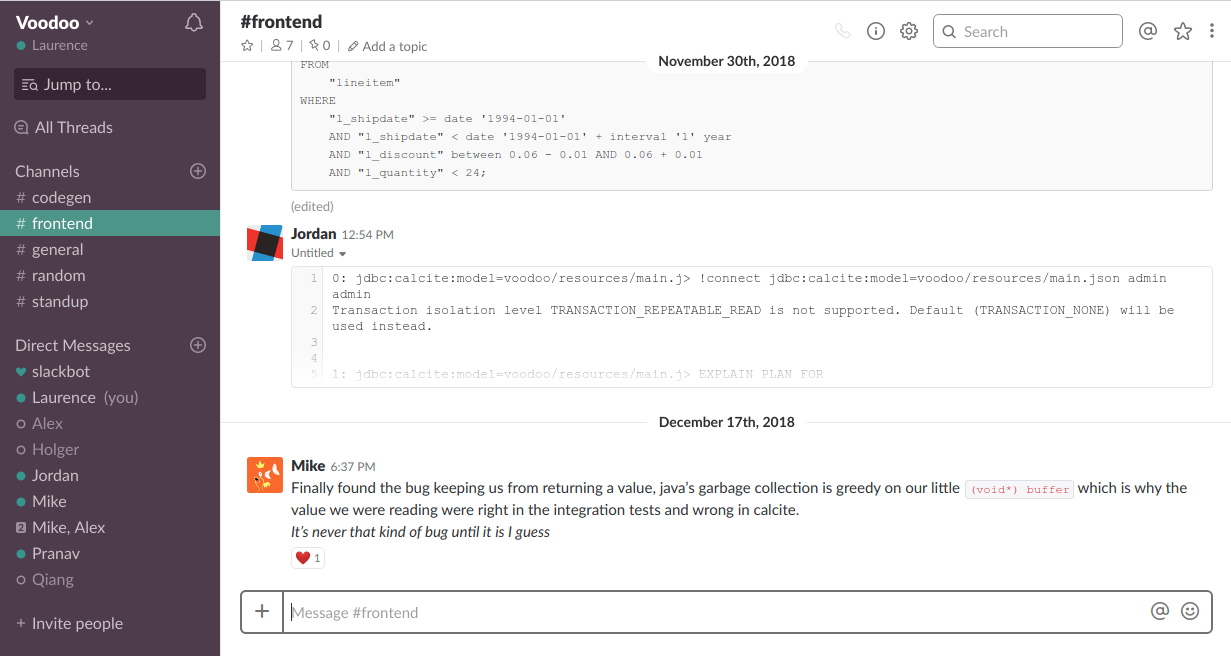
\includegraphics[width=0.9\linewidth]{project-management/slack.png}
    \caption{The \texttt{\#frontend} channel on Slack}
    \label{fig:slack}
\end{figure}

\newpage
\section{Software engineering practices and project planning}

\paragraph{eXtreme Programming} We used eXtreme programming \cite{XP:2013} based on the group's previous experience. The various checkpoints and the documentation which we are required to submit fit well into the project schedule. We met with our supervisor on every Friday of the checkpoint in order to come up with an iteration plan, reflecting on blockers and unfinished issues and figuring out which user stories (TPC-H queries) to integrate into the next plan. We could then write it down and submit it as documentation for each checkpoint, and share it on Slack with our supervisor. We would then use this to manipulate the GitLab issue board, making new issues, closing others, moving them between the different section, and making a new milestone to group those issues. We would then discuss how to assign them and how to organise the work for this checkpoint. A lot of independently created issues would appear during the checkpoints to be worked on in relevant time by anyone to pick. It could be bugs that were found, issues about improving some design, or work to do to improve developer productivity (and ultimately for the researchers/users who will use this project).

\paragraph{Stand-up meetings} To keep all team members updated on the current state of the project we held stand-up meetings. Not only for sharing the work that had been done and what was to be done next but also to seek help and form pair programming teams if something was blocking them. XP recommends daily meeting, but since this was not a full time project, we adapted daily stand-ups to bi-weekly stand-ups (on Mondays and Wednesdays). Whenever team members were unable to attend stand-ups (e.g. due to being away from university at holidays), we would still continue to hold standups through Messenger video calls.

\subsection{Project timeline}

We pivoted from another project in the middle of checkpoint 1 and met with our supervisor who explained to us the goals of the project that would serve as a release plan. We were given access to an existing codebase and the research paper for Voodoo. We summarise main goals of the iteration plan:

\paragraph{Checkpoint 1} 
After investigating and gaining familiarity with the existing Voodoo codebase and its concept, come up with a AST to represent the TPC-H query 6 code; code that we had to generate from the current codebase after making all the adjustments necessary to be able to compile and run the code on our systems.

\paragraph{Checkpoint 2}
Generate Voodoo vector algebra for TPC-H query 6 in Java using the existing \texttt{Printer} implementation after forming a Calcite plan tree. Investigate the best technology to code the AST from Checkpoint 1, and generate it using the most suitable one.

\paragraph{Checkpoint 3}
Generate Voodoo vector algebra for TPC-H query 1 and 19, and have query 6 running using the \texttt{ClangAst} back-end generating and running the right OpenCL code.

\paragraph{Checkpoint 4}
Generate and retrieve results for TPC-H queries 1, 6 and 19 by using a JDBC connection to Calcite by implementing an adapter, generate correct Voodoo and OpenCL code for them, and run OpenCL on the front-end data.

We implemented \emph{acceptance tests} from those objectives. For example automation of installation and CI work for checkpoint 1, use the printer implementation to check the correct output of the front-end in checkpoint 2, check the value of the result vector from a Voodoo program in checkpoint 3 and checking the value of a vector from an SQL query in checkpoint 4.

We expected there to be alterations to these objectives due to technical challenges we might face. We learned to plan according to our \emph{project velocity} with our supervisor, even using \emph{planning poker} as a way to better share our ideas on the time tasks would take. Communicating effectively with our supervisor during the iteration meetings was probably the biggest challenge but is something we have consistently became better at.

We chose to split the team into specialised groups due to the complexity and depth of the front-end and back-end code-bases: it required a fairly significant time investment to fully understand each component, and so we thought it would be unreasonable to expect all team members to be able to work on all components. As such, \textbf{Qiang} and \textbf{Jordan} developed the Calcite front-end, \textbf{Laurence} and \textbf{Alex} worked on the Voodoo back-end, and \textbf{Mayeul} and \textbf{Pranav} managed the good integration of the two sides and worked on issues that required knowledge of both the front-end and back-end.

A point to note is that due to the nature of the project, the first few tasks were long and required multiple team members working on a single task. However, as we improved our knowledge of the existing codebase and also improved the project structure, it was then possible for each individual group member to take ownership of various issues to fix and break down the separate tasks into smaller issues to fix - hence enabling us to improve our iteration time with more merge requests 
